\subsection{Приближённая интерполяция: метод наименьших квадратов.}

Интерполяция --- нахождение промежуточных значений по имеющемуся дискретному набору точных числовых значений. 

Постановка задачи интерполяции:

На отрезке $[a, b]$ в точках $\{x_1, x_2, \dotsc, x_n\}$ известны значения функции $f(x)$. Требуется построить функцию $g(x)$, совпадающую с заданной функцией $f(x)$ в этих точках.
\begin{equation*}
	g(x_k) = f(x_k), \, k = 1, 2, \dotsc, n.
\end{equation*}

Точки $\{x_1, x_2, \dotsc, x_n\}$ называются узлами интерполяции, а построение функции --- интерполированием. 

\textsc{Метод наименьших квадратов}

\begin{table}[H]
	\centering
	\begin{tabular}{|c|c|c|c|c|}
		\hline
		{$x$} & {$x_0$} & {$x_1$} & {$\dotsc$} & {$x_n$} \\ \hline 
		{$y$} & {$y_0$} & {$y_1$} & {$\dotsc$} & {$y_n$} \\ \hline 
	\end{tabular}
\end{table}

Задача: найти многочлен $f$.

$\deg{f} = m < n$.

Числа $y_k - f(x_k)$ называются невязками. 

Можно потребовать:
\begin{enumerate}
	\item Чтобы наибольшая по модулю невязка была как можно меньше;
	
	\item Чтобы сумма модулей невязок была как можно меньше;
	
	\item Чтобы сумма квадратов невязок была как можно меньше.
\end{enumerate}
\begin{gather*}
	f(x) = a_0 + a_1 x + a_2 x^2 + \dotsc + a_m x^m, \\
	\delta = \sum\limits_{k = 0}^{n}(y_{k} - a_0 - a_1 x - a_2 x^2 - \dotsc - a_m x^m)^2 \to \min \text{ --- многочлен 2 степени от } a_0, a_1, a_2, \dotsc, a_m; \\
	\frac{\partial \delta}{\partial a_0} = 0, \dotsc, \frac{\partial \delta}{\partial a_m} = 0 \text{ --- СЛАУ}.
\end{gather*}

\begin{example}
	Приведем пример из ДЗ №1, где было необходимо:
	\begin{quote}
		Для данной функции найти аппроксимирующую:
		\begin{enumerate}[label={\textbf{\alph*)}}, ref={\alph*}]
			\item линейную функцию,
			
			\item квадратичную функцию
		\end{enumerate}
		методом наименьших квадратов, выбрав для вычислений значения в концах отрезка всех целых точек внутри отрезка $[a, b]$.
	\end{quote} 
	
%	\paragraph{Дано.} 
	
	\begin{table}[H]
		\centering
		\begin{tabular}{|c||c|c|c|c|}
			\hline 
			$\mathbf{x}$ & 0 & 1 & 2 & 3 \\ \hline 
			$\mathbf{y}$ & 1 & -1 & 3 & 19 \\ \hline 
		\end{tabular}
	\end{table}
	\begin{equation*}
		\Phi(a_0, \dotsc, a_m) = \sum (a_0 + a_1 x_k + \dotsc + a_m x^m_k - y_k)^2 
	\end{equation*}
	
	\begin{enumerate}[label=\textbf{{\alph*)}}, ref={\alph*}]
		\item $f(x) = a_0 + a_1 x$
		
		\begin{align*}
			\Phi &= (a_0 - 1)^2 + (a_0 + a_1 + 1)^2 + (a_0 + 2 a_1 - 3)^2 + (a_0 + 3 a_1 - 19)^2 \\
			\frac{\partial \Phi}{\partial a_0} &= 2 (a_0 - 1) + 2 (a_0 + a_1 + 1) + 2 (a_0 + 2 a_1 - 3) + 2 (a_0 + 3 a_1 - 19) = 8 a_0 + 12 a_1 - 44 \\
			\frac{\partial \Phi}{\partial a_1} &= 2 (a_0 + a_1 + 1) + 4 (a_0 + 2 a_1 - 3) + 6 (a_0 + 3 a_1 - 19) = 12 a_0 + 28 a_1 - 124 
		\end{align*}
		
		\begin{equation*}
			\begin{cases}
				8 a_0 + 12 a_1 - 44 = 0 \\
				12 a_0 + 28 a_1 - 124 = 0
			\end{cases} \quad 
			\begin{cases}
				a_0 = -\frac{16}{5} \\
				a_1 = \frac{29}{5} 
			\end{cases}
		\end{equation*}
		
		Получаем, что: $f(x) = -\frac{16}{5} + \frac{29}{5} x$.
		
		\begin{figure}[H]
			\centering
			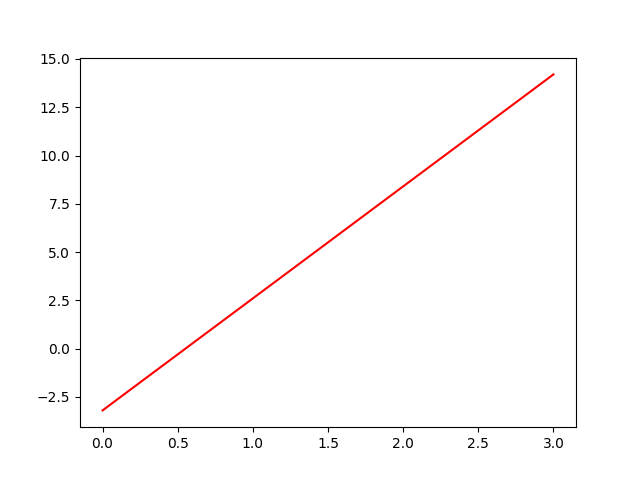
\includegraphics[scale=0.65]{img/1a.png}
		\end{figure}
		
		\item $f(x) = a_0 + a_1 x + a_2 x^2$
		
		\begin{align*}
			\Phi &= (a_0 - 1)^2 + (a_0 + a_1 + a_2 + 1)^2 + (a_ 0 + 2 a_1 + 4 a_2 - 3)^2 + (a_0 + 3 a_1 + 9 a_2 - 19)^2 \\
			\frac{\partial \Phi}{\partial a_0} &= 2 (a_0 - 1) + 2 (a_0 + a_1 + a_2 + 1) + 2 (a_0 + 2 a_1 + 4 a_2 - 3) + 2 (a_0 + 3 a_1 + 9 a_2 - 19) = \\ &= 8 a_0 + 12 a_1 + 28 a_2 - 44 \\
			\frac{\partial \Phi}{\partial a_1} &= 2 (a_0 + a_1 + a_2 + 1) + 4 (a_0 + 2 a_1 + 4 a_2 - 3) + 6 (a_0 + 3 a_1 + 9 a_2 - 19) = \\ &= 12 a_0 + 28 a_1 + 72 a_2 - 124 \\
			\frac{\partial \Phi}{\partial a_2} &= 2 (a_0 + a_1 + a_2 +1) + 8 (a_0 + 2 a_1 + 4 a_2 - 3) + 18 (a_0 + 3 a_1 + 9 a_2 - 19) = \\ &= 28 a_0 + 72 a_1 + 196 a_2 - 364
		\end{align*}
		
		\begin{equation*}
			\begin{cases}
				8 a_0 + 12 a_1 + 28 a_2 - 44 = 0 \\
				12 a_0 + 28 a_1 + 72 a_2 - 124 = 0 \\
				28 a_0 + 72 a_1 + 196 a_2 - 364 = 0
			\end{cases} \quad 
			\begin{cases}
				a = \frac{13}{10} \\
				b = - \frac{77}{10} \\ 
				c = \frac{9}{2}
			\end{cases}
		\end{equation*}
		
		Получаем, что $f(x) = \frac{13}{10} - \frac{77}{10} x + \frac{9}{2} x^2$.
		
		\begin{figure}[H]
			\centering
			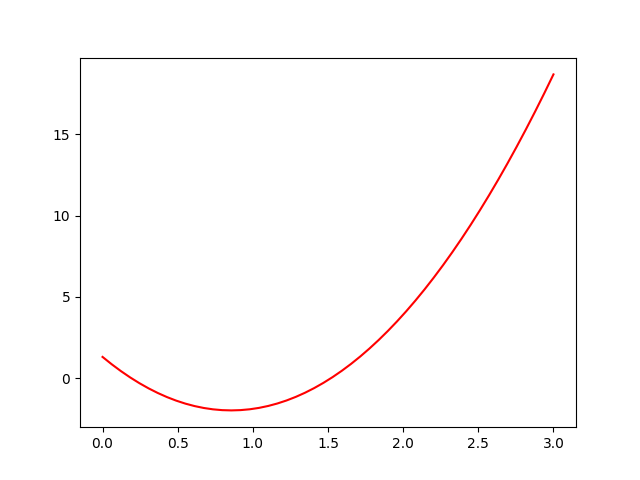
\includegraphics[scale=0.65]{img/1b.png}
		\end{figure}
	\end{enumerate} 
\end{example}